\begin{frame}{}
    \begin{center}
        \LARGE Introducci\'on y Marco Te\'orico
    \end{center}
\end{frame}

\begin{frame}{Evidencias de materia oscura.}
\begin{figure}
\centering
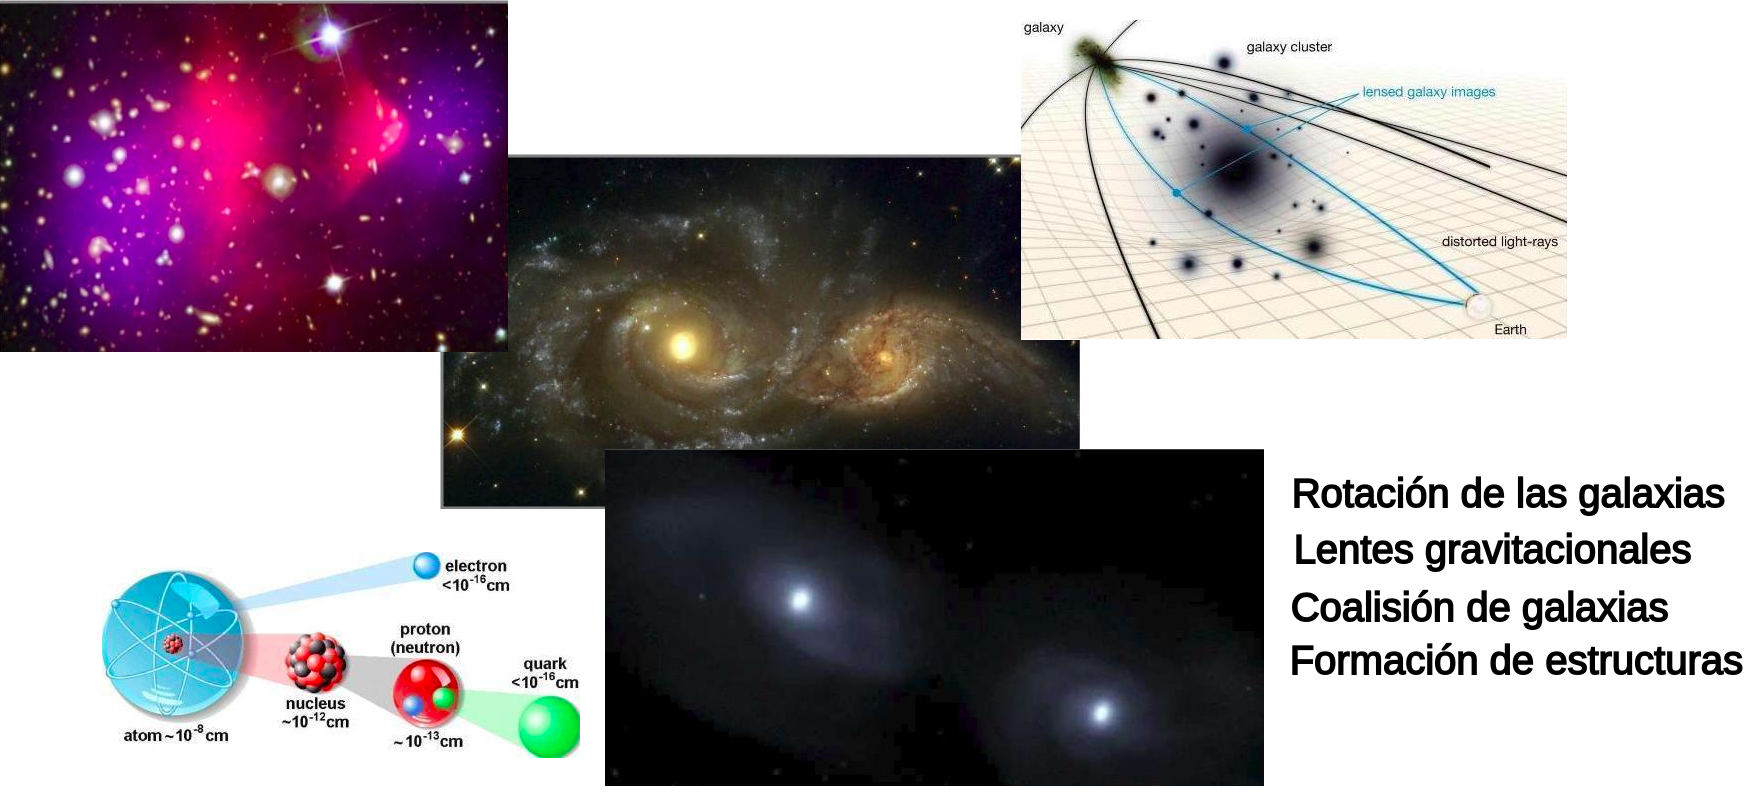
\includegraphics[width=1\textwidth]{Imag/materia_oscura.png}
\end{figure}

\end{frame}


% Teoria que describe la materia bariónica
\begin{frame}{Modelo Est\'andar}

\begin{figure}
\centering
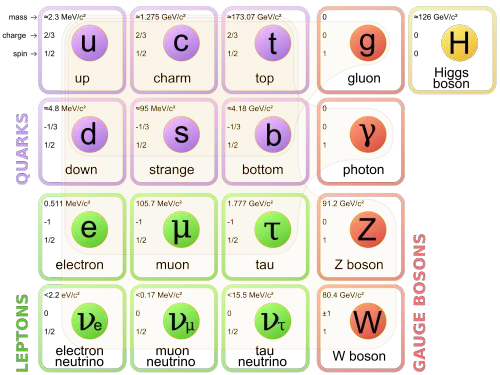
\includegraphics[width=.6\textwidth]{Imag/standard_model.png}
\caption{Modelo est\'andar de la f\'isica de las part\'iculas elementales.}
\end{figure}


\end{frame}



% Teoria que describe la materia bariónica
\begin{frame}{Modelo Est\'andar. Lagrangiano.}

\begin{columns}
\begin{column}{0.35\textwidth}
\Large{
\begin{align*}
\mathcal{L} &= - \frac{1}{4} F_{\mu \nu} F^{\mu \nu} \\
    &\phantom{{}=}+ i \bar{\psi} \cancel{D} \psi + h.c. \\
    &\phantom{{}=}+ \bar{\psi}_i y_{ij} \psi_j \phi + h.c. \\
    &\phantom{{}=}+ |D_\mu \phi|^2 - V(\phi)
\end{align*}
}
\end{column}
\begin{column}{0.65\textwidth}  %%<--- here
    \begin{itemize}
        \item Primera linea describe las fuerzas elementales electromagnetismo, fuerza nuclear debil y fuerte)
        \item La segunda linea describe como las fuerzas actu\'an en las particulas fundamentales (quarks y leptones)
        \item Tercera linea describe como las particulas obtienen sus masas del bos\'on de Higgs 
        \item La cuarta linea describe el campo de Higgs
    \end{itemize}
\end{column}
\end{columns}
\end{frame}


\begin{frame}{Mas alla del modelo est\'andar}

El modelo est\'andar describe de forma exitosa como funciona el universo sin embargo falla en dar explicaci\'on a fen\'omenos tales como:

\begin{itemize}
    \item Descripci\'on cuantica de la fuerza de gravedad
    \item \textbf{Materia Oscura: Por observaciones cosmologicas se sabe que el modelo est\'andar solo contempla el 5\% de la energia presente en el universo.  Cerca de 26\% debe de ser materia oscura, la cual solo interactua debilmente con los campos del modelo est\'andar. El modelo est\'andar no contempla particulas fundamentales como constituyentes de la materia oscura}
    \item Energia Oscura
    \item Masa del neutrino
    \item Asimetria materia-Antimateria
\end{itemize}
    
\end{frame}



\begin{frame}{Mas alla del modelo est\'andar. Modelo Dark-SUSY.}

\begin{itemize}
\item La materia oscura esta compuesta de particulas fundamentales 
\item Estas particulas estan descritas por un formalismo te\'orico parecido al del modelo est\'andar (Teoria cu\'antica de campo) 
\item Que estas nuevas particulas puedan ser producidas por medio de la colisi\'on de protones altamente energ\'eticos (como las producidas en el Gran Acelerador de Hadrones)
\end{itemize}

\begin{figure}
\centering
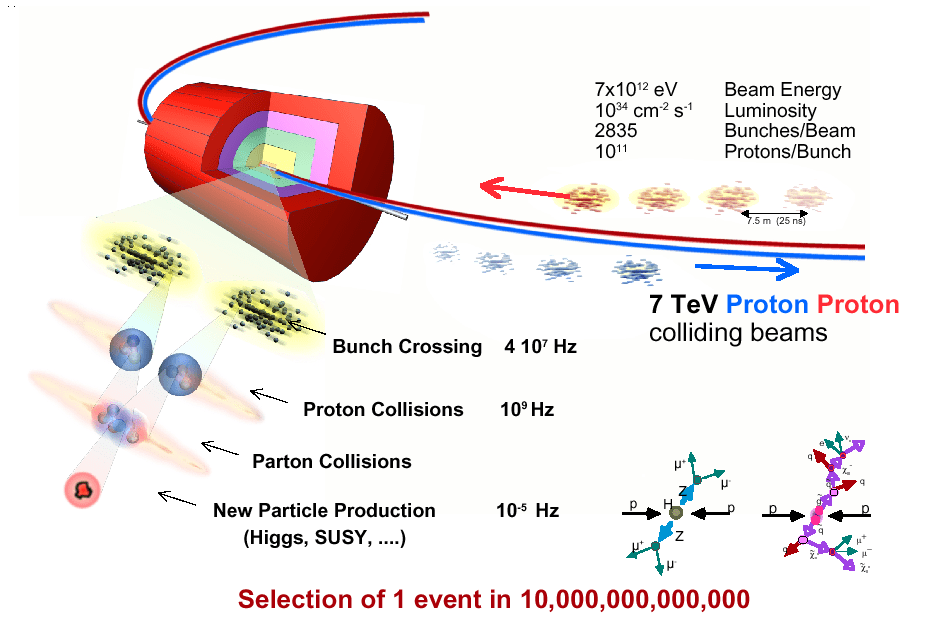
\includegraphics[width=.3\textwidth]{Imag/sketch_collisions.png}
%    \caption{Representac\'on de las colisiones en el Gran Colisionador de Hadrones}
\end{figure}
    
\end{frame}



\begin{frame}{Mas alla del modelo est\'andar. Modelo Dark-SUSY.}
Las nuevas fuerzas en el escenario Dark-SUSY puede asociarse al modelo est\'andar por medio de un termino de mezcla (kinetic mixing) que en forma de lagrangia tiene la siguiente forma: 

\begin{align*}
\mathcal{L}_{KM} &= - \frac{\epsilon}{2} F^{Y}_{\mu \nu} F^{D_{\mu \nu}} 
\end{align*} 

donde $F^{Y}_{\mu nu} = \partial_{\nu}A_{\nu}^{D} - \partial_{\nu}A_{\nu}^{D}$ es el campo de fuerzas en el sector oscuro. El rango tipico de $\epsilon$ es en el rango $10^{-8}$ - $10^{-2}$.
    
\end{frame}



\begin{frame}{Mas alla del modelo est\'andar. Modelo Dark-SUSY}
\begin{itemize}
\item Producci\'on de fotones oscuros por medio del portal del Higgs.
\item En este modelo el Higgs decae a particulas supersim\'etricas (neutralinos $n_{1}$)
\item subsequentemente cada neutralino decae a un neutralino oscuro ($n_{D}$) y un fot\'on oscuro ($\gamma_{D}$)
\item Cada fot\'on oscuro decae a un par de muones de carga opuesta\end{itemize}
\begin{figure}
\centering
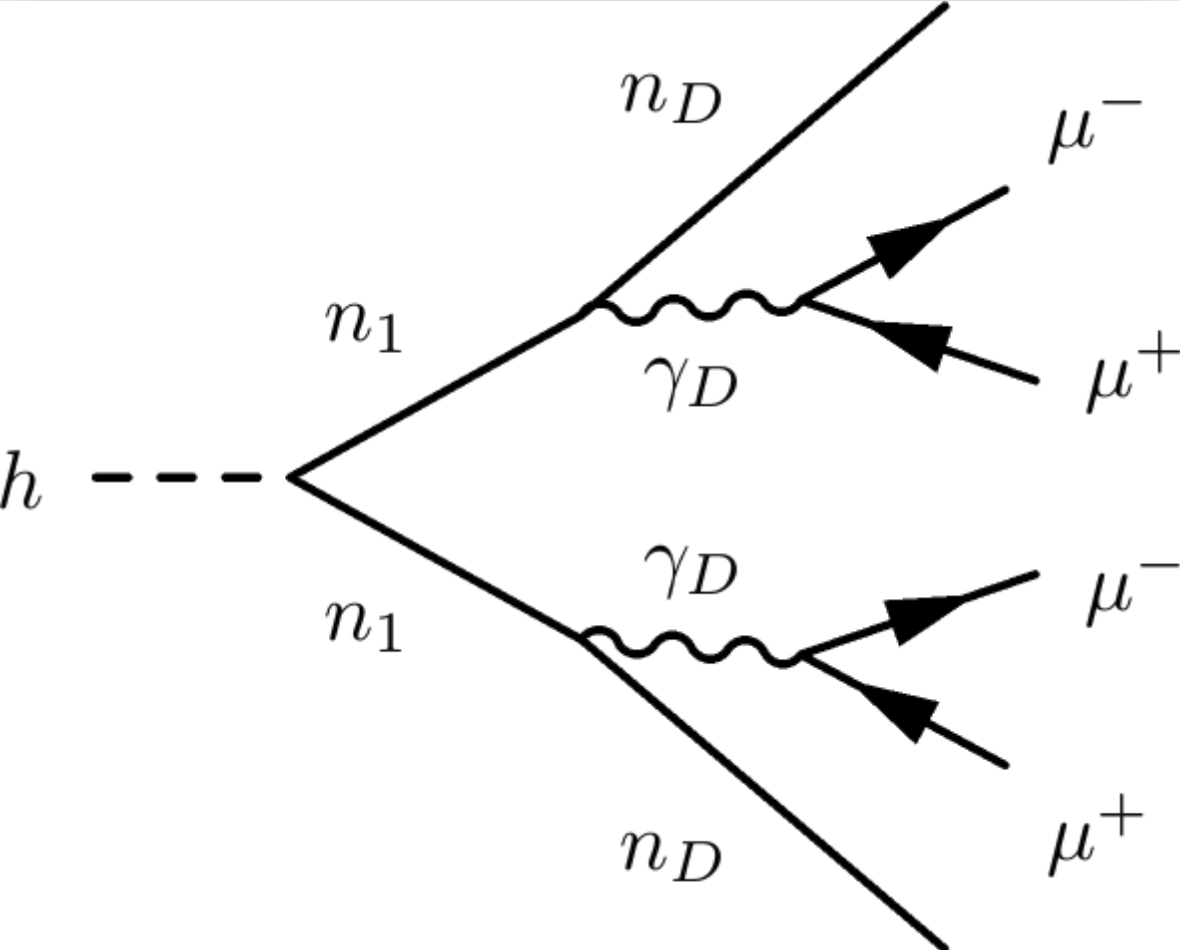
\includegraphics[width=.3\textwidth]{Imag/decae.png}
\caption{Diagrama de Feynman del modelo Dark-SUSY}
\end{figure}

\end{frame}

\begin{frame}{Mas alla del modelo est\'andar. Modelo Dark-SUSY}
Decaimiento del foton oscuro a leptones
\begin{itemize}
\item Debido al factor de mezcla $\epsilon$ el foton oscuro decae a leptones del modelo estandar con una anchura parcial dada por la siguiente expresion: 
\begin{equation}
\Gamma_{\gamma_{D}}\rightarrow \bar{l}l =\frac{1}{3}\alpha\epsilon^{2}m_{\gamma_{D}}\sqrt{1-\frac{4m_{l}^{2}}{m_{\gamma_{D}}^{2}}}\left(1+\frac{2m_{l}^{2}}{m_{\gamma_{D}}^{2}}\right)
\end{equation}

\end{itemize}
Donde $m_{l}$ es la masa del lepton (e,$\mu$, or $\tau$)    
\end{frame}


\begin{frame}{Mas alla del modelo est\'andar. Modelo Dark-SUSY}
Tiempo de vida\\
\begin{itemize}
\item El tiempo de vida esta relacionado a la anchura de decaimiento con la siguiente expresi\'on
\end{itemize}
\begin{equation}
\tau_{\gamma_{D}} = \frac{\hbar}{\Gamma_{\gamma_{D}}} \Rightarrow 
\tau_{\gamma_{D}}(\epsilon, m_{\gamma_{D}}) = \frac{1}{\epsilon^{2}}\times f(m_{\gamma_{D}})
\end{equation}
Es decir el tiempo de vida es una funci\'on de la masa del fot\'on oscuro y el par\'ametro de mezcla $\epsilon$. 

Es conveniente expresar el tiempo de vida como una distancia $c\tau_{\gamma_{D}}$, donde c es la velocidad de la luz. Tambi\'en es conveniente medir $c\tau_{\gamma_{D}}$ en milímetros para relacionar la sensitividad del modelo en el an\'alisis de datos. 
\begin{equation}
c\tau_{\gamma_{D}}(\epsilon,m_{\gamma_{D}})[mm] = \frac{c[mm/s]\times \hbar[GeV.s]}{\epsilon^{2}} \times f(m_{\gamma_{D}}[GeV^{-1}]
\end{equation}
\end{frame}


\begin{frame}{Propiedades del modelo}
\begin{figure}[ht]

\begin{minipage}[b]{0.45\linewidth}
\centering
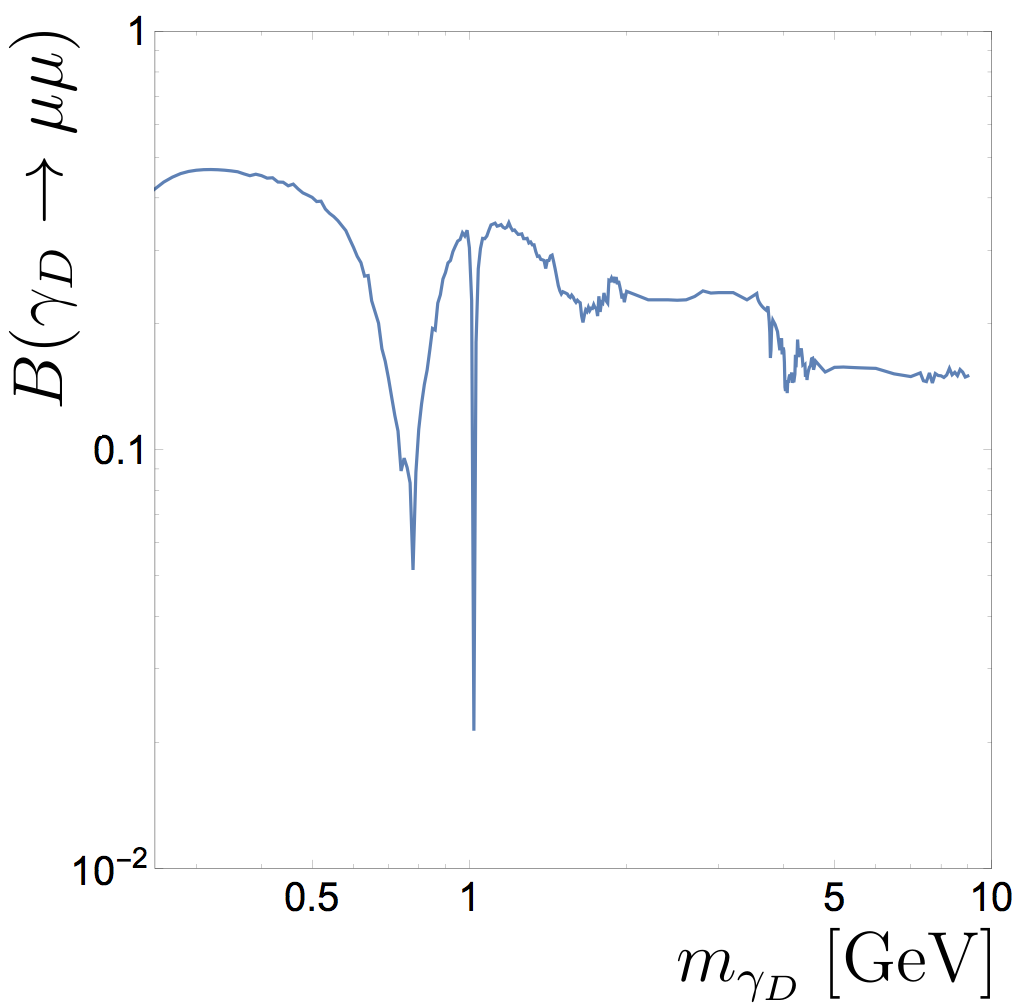
\includegraphics[width=1\textwidth]{Imag/teoria_dark_photon2.png}
\caption{Probabilidad de decaimiento del fotos oscuro a dos muones}
\end{minipage}
\hspace{0.5cm}
\begin{minipage}[b]{0.45\linewidth}
\centering
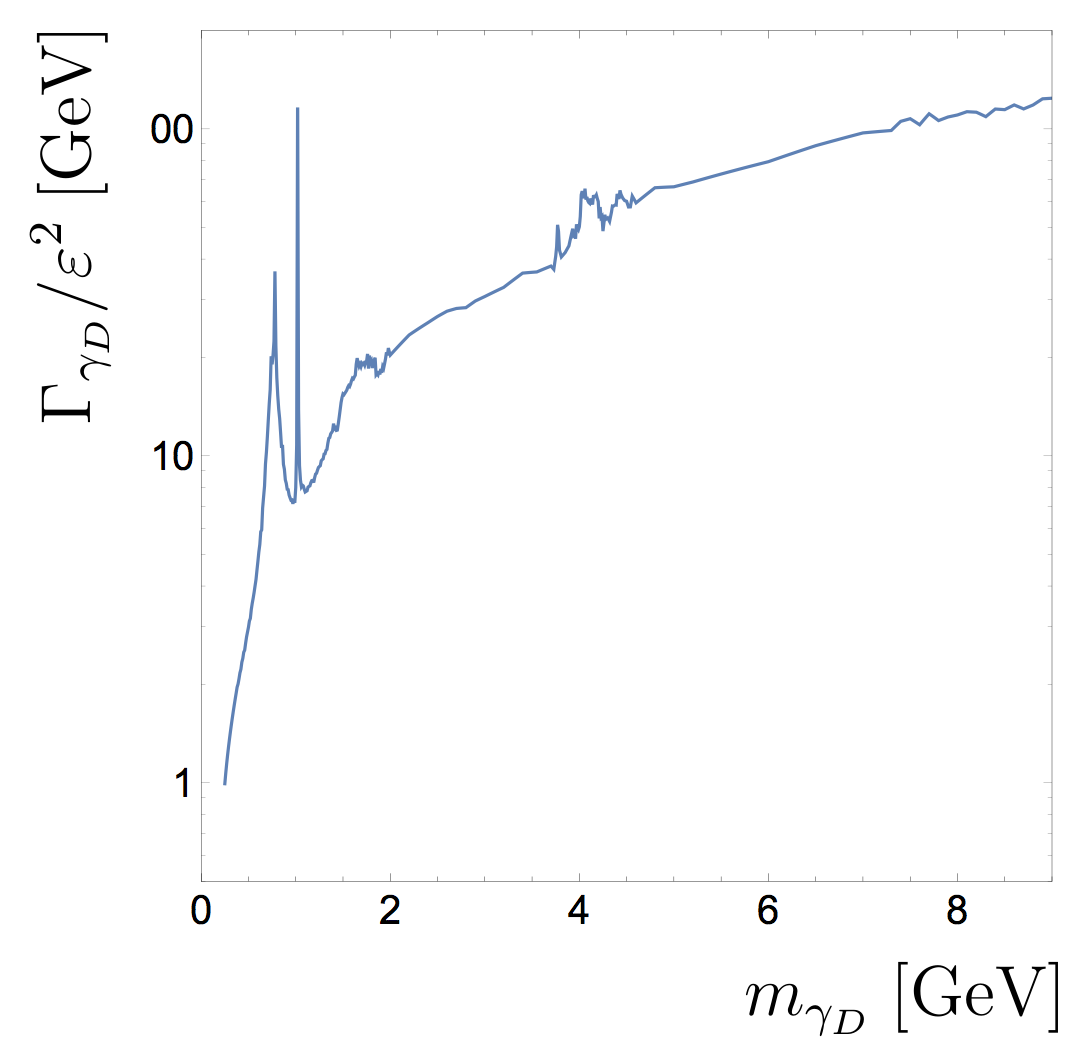
\includegraphics[width=1\textwidth]{Imag/teoria_dark_photon1.png}
\caption{Amplitud del decaimiento dividido por el coeficiente de mezcla cinetico}
\end{minipage}
\end{figure}
\end{frame}




% Teoría que intenta describir la existencia de materia oscura
% PROBLEMA, PROBLEMA, PROBLEMA, PROBLEMA, PROBLEMA
\begin{frame}{Problema de la investigaci\'on.}
%Dado que el modelo est\'andar no describe de forma \'exitosa como funciona el universo, part\'iculas hipot\'eticas derivadas de teor\'ias alternativas son necesarias para explicar estos fen\'omenos, y se hace necesario identificar la teoría desde limitaciones de los detectores.

Actualmente los modelos te\'oricos que predicen la formaci\'on de nuevas part\'iculas de materia oscura no han sido explorados ampliamente, por lo que no hay muchos m\'etodos desarrollados de identificaci\'on y caracterizaci\'on de las posibles se\~nales que ayuden a optimizar el proceso de calibraci\'on cuando se logre alcanzar el espacio fase de estos modelos.

\end{frame}


% HIPOTESIS, HIPOTESIS, HIPOTESIS, HIPOTESIS, HIPOTESIS
\begin{frame}{Hip\'otesis}
Si se hace supuesto que la materia oscura est\'a descrita por la teor\'ia MSSMD, al reconstruir la se\~nal desde los detectores por medio de la simulaci\'on es posible crear m\'etodos flexibles y eficientes de caracterizaci\'on, idenficaci\'on y reconstrucci\'on de las part\'iculas hipot\'eticas predichas por la teor\'ia.
\end{frame}


\begin{frame}{Objetivo General}
Estudiar por medio de simulaci\'on de Monte Carlo el modelo te\'orico ``Dark Susy'', reconstruyendo te\'oricamente las propiedades del fot\'on oscuro en un entorno simulado de los detectores que realizar\'ian la detecci\'on en configuraciones experimento CMS llamada Run-2 y en Alta Luminosidad.

\end{frame}


\begin{frame}{Objetivos espec\'ificos.}

\begin{itemize}
\item Recreaci\'on de la teor\'ia por medio de simulaci\'on mediante el desarrollo de un entorno de simulaci\'on y an\'alisis usando los recursos computacionales de la Universidad de Sonora (ACARUS).
%Estudio por medio de simulaci\'on de un modelo te\'orico que predice la creaci\'on de nuevas part\'iculas y fuerzas fundamentales.
%\item Dichas part\'iculas conocidas como fotones oscuros (Dark photons) son uno de los candidatos para explicar la composici\'on de la materia oscura en el universo.
\item Desarrollo de m\'etodos de identificaci\'on de la se\~nal a caracterizar.
\item Caracterizar la se\~nal en cuesti\'on y sus propiedades en el contexto del experimento CMS y sus futuras actualizaciones.
\end{itemize}
\end{frame}

